\documentclass{standalone}
\usepackage{tikz}
\renewcommand{\familydefault}{\sfdefault}
\usetikzlibrary{arrows}
\tikzstyle{every node}=[minimum width=12ex, node distance=3cm]

\tikzset{>=stealth'}
\begin{document}
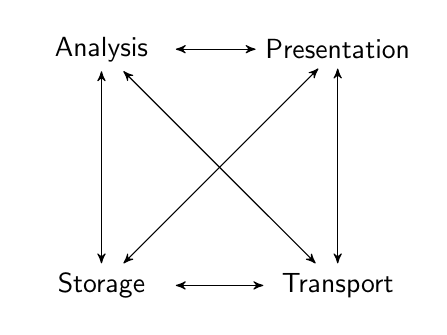
\begin{tikzpicture}
\node (presentation) [] {Presentation};
\node (analyses)     [left of = presentation] {Analysis};
\node (transport)    [below of = presentation] {Transport};
\node (storage)      [left of = transport] {Storage};

\draw [<->] (presentation) -- (transport);
\draw [<->] (presentation) -- (storage);
\draw [<->] (presentation) -- (analyses);
\draw [<->] (analyses)     -- (storage);
\draw [<->] (analyses)     -- (transport);
\draw [<->] (storage)      -- (transport);
      
\end{tikzpicture}
\end{document}
